\begin{figure*}[t]
\centering
\begin{subfigure}{.196\linewidth}
\centering
\raisebox{0cm}{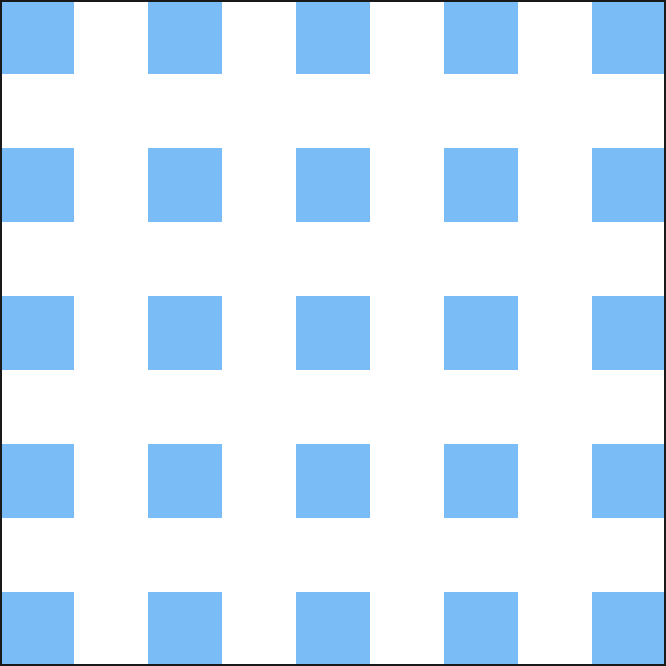
\includegraphics[width=\linewidth]{figures/2d/sparse_checkerboard.pdf}}
\caption{Train Distribution}\label{fig:2d_sparse_checkerboard}
\end{subfigure}
\hspace{-0.15cm}
\begin{subfigure}{.196\linewidth}
\centering
\raisebox{0cm}{\includegraphics[width=\linewidth]{figures/2d/char_scatter.pdf}}
\caption{Char Model Pred.}\label{fig:2d_char_scatter}
\end{subfigure}
\hspace{-0.15cm}
\begin{subfigure}{.196\linewidth}
\centering
\raisebox{0cm}{\includegraphics[width=\linewidth]{figures/2d/float_scatter.pdf}}
\caption{Float Model Pred.}\label{fig:2d_float_scatter}
\end{subfigure}
\begin{subfigure}{.196\linewidth}
\centering
\raisebox{0.0cm}{\includegraphics[width=\linewidth]{figures/2d/bar.pdf}}
\caption{ID--OOD}
\label{fig:2d_bar}
\end{subfigure}
\hfill
\begin{subfigure}{.196\linewidth}
\centering
\includegraphics[width=\linewidth]{figures/2d/dynamics.pdf}
\caption{Dynamics}
\label{fig:2d_dynamics}
\end{subfigure}
\caption{\textbf{2D Parameter-Space Generalization.} (\cref{sssection:2d})
(a) Training positions are sampled from the checkerboard.
When evaluated on images with uniformly sampled positions, the char-based model fails to generalize outside the training distribution (b) while the float-based model effectively interpolates samples (c).
Randomly-sampled testing locations are shown in red and the corresponding predictions in blue.
(d) shows that while both methods well-estimate samples from the ID condition, the char-based model struggles to generalize.
(e) shows a plot of the model's validation MSE as a function of the number of training steps.
We observe that the training of the float-based model is much smoother and converges quickly.
}
\label{fig:2d}
\end{figure*}